\documentclass[10pt]{article}
\usepackage[russian]{babel}
\usepackage[utf8]{inputenc}
\usepackage[T2A]{fontenc}
\usepackage{amsmath}
\usepackage{amsfonts}
\usepackage{amssymb}
\usepackage[version=4]{mhchem}
\usepackage{stmaryrd}
\usepackage{graphicx}
\usepackage[export]{adjustbox}
\graphicspath{ {./images/} }

%New command to display footnote whose markers will always be hidden
\let\svthefootnote\thefootnote
\newcommand\blfootnotetext[1]{%
  \let\thefootnote\relax\footnote{#1}%
  \addtocounter{footnote}{-1}%
  \let\thefootnote\svthefootnote%
}

%Overriding the \footnotetext command to hide the marker if its value is `0`
\let\svfootnotetext\footnotetext
\renewcommand\footnotetext[2][?]{%
  \if\relax#1\relax%
    \ifnum\value{footnote}=0\blfootnotetext{#2}\else\svfootnotetext{#2}\fi%
  \else%
    \if?#1\ifnum\value{footnote}=0\blfootnotetext{#2}\else\svfootnotetext{#2}\fi%
    \else\svfootnotetext[#1]{#2}\fi%
  \fi
}

\begin{document}

\section*{§ 3. Пример: нелинейный маятник •}
Описываемые здесь и далее три модели дают некоторое представление о возможных видах нелинейных колебаний в случае одной степени свободы, но далеко не исчерпывают всего их разнообразия.

Траектории нелинейного маятника. Гамильтониан нелинейного маятника с единичной массой имеет вид


\begin{equation*}
H=1 / 2 \dot{x}^{2}-\omega_{0}^{2} \cos x, \tag{3.1}
\end{equation*}


где $q=x$ и $p=\dot{x}$. Уравнения движения (1.5) дают


\begin{equation*}
\ddot{x}+\omega_{0}^{2} \sin x=0 . \tag{3.2}
\end{equation*}


Потенциал $V=-\omega_{0}^{2} \cos x$ и фазовый портрет приведены на рис. 1.10.\\
Аналогично уравнениям (2.4) состояния равновесия маятника определяются уравнениями


\begin{equation*}
\dot{x}_{s}=0, \quad \sin x_{s}=0 . \tag{3.3}
\end{equation*}


Это дает $\dot{x}_{s}=0, x_{s}=\pi n, n=0, \pm 1, \ldots$ В положении равновесия скорость $\dot{x}_{s}$ равна нулю, а потенциал $V\left(x_{s}\right)$ имеет минимум (четные $n$ ) или максимум (нечетные $n$ ). Соответственно точки при четных $n$-эллиптические, при нечетных $n$-гиперболические.

Траектории на фазовой плоскости при $H<\omega_{0}^{2}$ соответствуют «захваченным» частицам, совершающим финитные колебания в потенциальных ямах. При $H>\omega_{0}^{2}$ фазовые траектории относятся к «пролетным» частицам, движение которых инфинитно. Как видно из рис. 1.10, это периодические колебания около некоторого значения скорости, причем верхней и нижней ветвям фазовых кривых соответствуют различные направления скорости.

Сепаратрисой является фазовая траектория, проходящая через точку $\dot{x}_{s}=0, x_{s}=\pi$. Поэтому ей соответствует энергия $H_{s}=\omega_{0}^{2}$. Решение на сепаратрисе найти просто. Действительно, подставим $H_{s}=\omega_{0}^{2}$ в уравнение (3.1) и выразим из него $\dot{x}$ :


\begin{equation*}
\dot{x}= \pm 2 \omega_{0} \cos (x / 2) . \tag{3.4}
\end{equation*}


Отсюда интегрирование при начальном условии $t=0, x=0$ дает


\begin{equation*}
\omega_{0} t=\ln \operatorname{tg}\left(\frac{x}{4}+\frac{\pi}{4}\right), \tag{3.5}
\end{equation*}


или


\begin{equation*}
x=4 \operatorname{arctg} e^{\omega_{0} t}-\pi . \tag{3.6}
\end{equation*}


Выражение (3.6) есть не что иное, как уравнение сепаратрисы (вторая ветвь сепаратрисы получается из первой (3.6) обращением времени $t \rightarrow-t$ ).

Однако более интересная информация о динамике частицы на сепаратрисе получается, если рассмотреть выражение для скорости $v=\dot{x}$. Для этого из (3.5) получаем соотношение

$$
\cos (x / 2)=1 / \operatorname{ch}\left(\omega_{0} t\right)
$$

и подставляем его в (3.4):


\begin{equation*}
v= \pm 2 \omega_{0} / \operatorname{ch}\left(\omega_{0} t\right) \tag{3.7}
\end{equation*}


\begin{center}
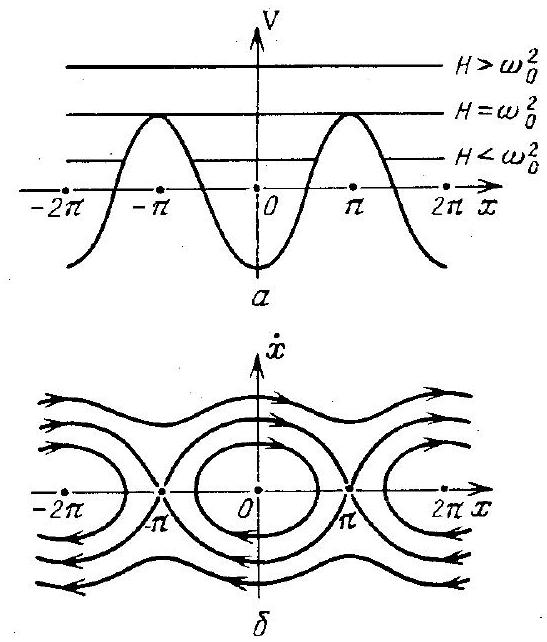
\includegraphics[max width=\textwidth]{2024_12_13_2abbd56e24043f80c30dg-2(1)}
\end{center}

Рис. 1.10. Периодический потенциал (a) и соответствующий ему фазовый портрет (б)

Решение типа (3.7) имеет вид уединенной волны (рис. 1.11) и носит название солитона. Характерная ширина профиля скорости $\sim 1 / \omega_{0}$. Его края экспоненциально спадают при $t \rightarrow \pm \infty$. Знак плюс в (3.7) соответствует солитону, движущемуся вправо (верхняя ветвь сепаратрисы на фазовой плоскости - рис. 1.10б). Знак минус в (3.7) соответствует движению влево.

Рассмотрим теперь общее решение уравнения (3.2) при тех же начальных условиях $t=0, x=0$. Для удобства воспользуемся переменными действие-угол, определенными формулами (2.7). Введем параметр *) $x$ :\\
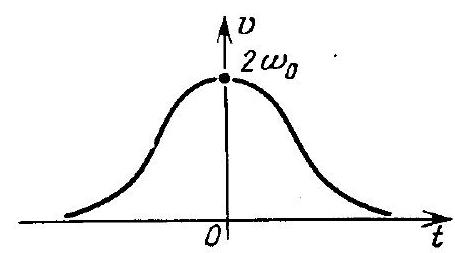
\includegraphics[max width=\textwidth, center]{2024_12_13_2abbd56e24043f80c30dg-2}

Рис. 1.11. Солитоноподобное решение для скорости на сепаратрисе


\begin{equation*}
x^{2}=\left(\omega_{0}^{2}+H\right) / 2 \omega_{0}^{2}=1 / 2\left(1+H / \omega_{0}^{2}\right), \tag{3.8}
\end{equation*}


принимающий на сепаратрисе значение 1 и изменяющийся в области $[0, \infty)$, и переменную $\xi$ :


\begin{align*}
x \sin \xi=\sin (x / 2) & (x \leqslant 1),  \tag{3.9}\\
\sin \xi=\sin (x / 2) & (x \geqslant 1) .
\end{align*}


Имеем

$$
I=I(H)=\frac{2}{\pi} \int_{0}^{x_{0}} d x\left[2\left(H+\omega_{0}^{2} \cos x\right)\right]^{1 / 2}
$$

\footnotetext{*) Здесь и далее одна и та же буква $H$ используется как для обозначения гамильтониана, так и для интеграла энергии всюду, где это не должно вызвать недоразумений.
}где точка поворота $x_{0}$ находится из условия

$$
H+\omega_{0}^{2} \cos x_{0}=0
$$

и использована симметрия движения частицы при определении интеграла $I(H)$. Здесь возникает необходимость доопределить выражение (2.7) для $I$ при значениях параметра $x^{2}>1$. Действительно, в этом случае из (3.8) следует, что уравнение для точки поворота не имеет решения, и в качестве точки $x_{0}$ в интеграле для $I$ следует взять $x_{0}=\pi$. При таком определении действие есть площадь, ограниченная по $x$ областью (- $-\pi$ ) (см. рис. 1.10б) и лежащая между верхней и нижней относительно сепаратрисы ветвями траектории. Именно такое определение позволяет произвести непрерывную сшивку решения при переходе через сепаратрису (производная при этом имеет разрыв)

С помощью подстановки (3.9) приходим к выражению

\[
I(H)=\frac{8}{\pi} \omega_{0}\left\{\begin{array}{l}
E\left(\frac{\pi}{2} ; x\right)-\left(1-x^{2}\right) F\left(\frac{\pi}{2} ; x\right) \quad(x \leqslant 1),  \tag{3.10}\\
x E\left(\frac{\pi}{2} ; \frac{1}{x}\right) \quad(x \geqslant 1)
\end{array}\right.
\]

где $F(\pi / 2 ; x)$ и $E(\pi / 2 ; x)$ - полные эллиптические интегралы соответственно первого и второго рода.

Из (3.10) сразу находим частоту нелинейных колебаний маятника:


\begin{equation*}
\omega(H)=\frac{d H(I)}{d I}=\left[\frac{d I(H)}{d H}\right]^{-\mathbf{1}} \tag{3.11}
\end{equation*}


Используя свойства эллиптических интегралов, находим

\[
\omega(H)=\frac{\pi}{2} \omega_{0} \begin{cases}\frac{1}{F(\pi / 2 ; x)} & (x \leqslant 1),  \tag{3.12}\\ \frac{x}{F(\pi / 2 ; 1 / x)} & (x \geqslant 1) .\end{cases}
\]

Мы отложим исследование формулы (3.12) до следующего пункта, а сейчас продолжим нахождение решения.

Согласно определению $S(q, I)$ в формулах (2.7) имеем

\[
S(x, I)= \begin{cases}4 \omega_{0}\left[E(\xi ; x)-\left(1-x^{2}\right) F(\xi ; x)\right] & (x \leqslant 1),  \tag{3.13}\\ 4 \omega_{0} x E(\xi ; 1 / x) & (x \geqslant 1),\end{cases}
\]

где $\xi=\xi(x)$ определяется формулами (3.9). Нетрудно видеть, что полному интегралу по четверти периода движения соответствует точка $x_{0}$ такая, что

$$
\begin{array}{ll}
\sin \left(x_{0} / 2\right)=x^{2} & (x \leqslant 1) \\
\sin \left(x_{0} / 2\right)=1 & (x \geqslant 1)
\end{array}
$$

Отсюда в любом случае $\xi_{0}=\pi / 2$, и выражение $4 S\left(x_{0}, T\right) / 2 \pi$ переходит в формулы для действия (3.10), как это и должно быть.

Дифференцирование $S(x, I)$ по $I$ определяет фазовую переменную $\vartheta$ (см. (2.7)).

Из формулы (3.1) для $H$ и определения (3.9) находим скорость:

\[
\dot{x}=2 x \omega_{0}\left\{\begin{array}{ll}
\frac{\cos \xi}{1-\frac{1}{x^{2}} \sin ^{2} \xi}
\end{array}\right\}=2 x \omega_{0} \begin{cases}\operatorname{cn}(t ; x) & (x \leqslant 1),  \tag{3.14}\\
\operatorname{dn}\left(t ; \frac{1}{x}\right) & (x \geqslant 1),\end{cases}
\]

где cn и dn - эллиптические функции Якоби. При $x=1$ выражение (3.14) переходит в (3.7) (знаки $\pm$ для простоты опускаются).

Спектр нелинейного маятника. Нашей ближайшей целью будет понять качественный характер колебаний маятника для различных значений его энергии $H$. Для этого сделаем две вещи. Во-первых, введем число


\begin{equation*}
N=\frac{\omega_{0}}{\omega(H)}=\frac{2}{\pi} F\left(\frac{\pi}{2} ; x\right) \quad(x \leqslant 1) \tag{3.15}
\end{equation*}


и, во-вторых, разложим выражение (3.14) для $\dot{x}$ в ряд Фурье:

\[
\dot{x}=8 \omega \begin{cases}\sum_{n=1}^{\infty} \frac{a^{n-1 / 2}}{1+a^{2 n-1}} \cos [(2 n-1) \omega t] & (x \leqslant 1),  \tag{3.16}\\ 1 / 4+\sum_{n=1}^{\infty} \frac{a^{n}}{1+a^{2 n}} \cos (n \omega t) & (x \geqslant 1)\end{cases}
\]

где


\begin{align*}
& a=\exp \left(-\pi \frac{F^{\prime}}{F}\right), \quad F \equiv F\left(\frac{\pi}{2} ; \bar{x}\right), \\
& F^{\prime} \equiv F\left(\pi / 2 ; \sqrt{1-\bar{x}^{2}}\right), \quad \omega=\omega(H),  \tag{3.17}\\
& \bar{x}= \begin{cases}x & (x \leqslant 1), \\
1 / x & (x \geqslant 1) .\end{cases}
\end{align*}


Рассмотрим теперь различные асимптотики выражений (3.16) и (3.17). Воспользуемся следующими асимптотиками полного эллиптического интеграла $F(\pi / 2 ; x)$ :

\[
F\left(\frac{\pi}{2} ; x\right) \sim\left\{\begin{array}{l}
\pi / 2 \quad(x \ll 1),  \tag{3.18}\\
1 / 2 \ln \frac{32 H_{s}}{H_{s}-H} \quad\left(1-x^{2} \ll 1\right) .
\end{array}\right.
\]

Отсюда

\[
N \sim\left\{\begin{array}{l}
1 \quad(x \ll 1)  \tag{3.19}\\
\frac{1}{\pi} \ln \frac{32 H_{s}}{H_{s}-H}
\end{array} \quad\left(1-x^{2} \ll 1\right) .\right.
\]

Аналогично из (3.17), (3.18) и (3.15) находим

\[
a \sim\left\{\begin{array}{l}
x^{2} / 32 \quad(x \ll 1),  \tag{3.20}\\
\exp (-\pi / N) \quad\left(1-x^{2} \ll 1\right) .
\end{array}\right.
\]

Теперь легко определить характер колебаний маятника во всех областях. При $x \ll 1$, т. е. при очень малых энергиях системы, частота $\omega(H) \sim \omega_{0}$ и $N \sim 1$. Кроме того, согласно (3.20) амплитуды $а$ малы. Поэтому в (3.16) имеет смысл оставить только первое слагаемое суммы, так как малость остальных нарастает с ростом $n$. Это дает

$$
v=\dot{x} \approx \omega_{0} \sqrt{2 x^{2}} \cos \left(\omega_{0} t\right)=\sqrt{2 \omega_{0} I} \cos \left(\omega_{0} t\right)
$$

в соответствии с обычной линейной теорией (действительно, энергия, отсчитываемая от дна потенциальной ямы, равна $\delta H=\omega_{0}^{2}+H$, и $I=\delta H / \omega_{0}=$ $\left.=x^{2} H_{s} / \omega_{0}=x^{2} \omega_{0}\right)$.

Пусть теперь $x^{2} \rightarrow 1$, т. е. $H \rightarrow H_{s}$. Тогда вблизи сепаратрисы частота $\omega(H) \longrightarrow 0$, а период колебаний логарифмически расходится (см. (3.19)). Скорость $\dot{x}$ системы приближается к пе• риодической последовательности солитоноподобных импульсов (рис. 1.12). Расстояние между двумя горбами в одной и той же фазе близко к периоду колебаний $2 \pi / \omega(H)$, а ширина каждого горба близка к $2 \pi / \omega_{0}$. Поэтому число $N$\\
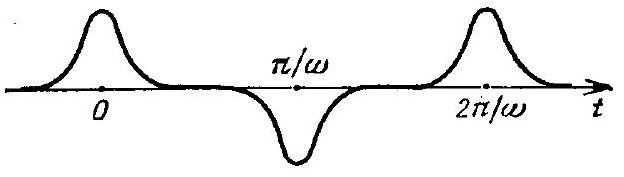
\includegraphics[max width=\textwidth, center]{2024_12_13_2abbd56e24043f80c30dg-4}

Рис. 1.12. Зависимость скорости от времени вблизи сепаратрисы

определяет «скважность» функции $v(t)$. Вводя спектр скорости, как в (2.11), видим, согласно (3.20) и (3.16), что при $N \gg 1$, т. е. вблизи сепаратрисы,

$$
b_{n}=8 \omega \frac{a^{n-1 / 2}}{1+a^{2 n-1}}
$$

Принимая во внимание выражение для $a$ в (3.20) при $1-x^{2} \ll 1$, получаем

\[
b_{n} \sim 8 \omega\left\{\begin{array}{l}
1 \quad(1<n \leqslant N)  \tag{3.21}\\
\exp (-\pi n / N) \quad(n]>[N)
\end{array}\right.
\]

т. е. все амплитуды приблизительно равны вплоть до $n \sim N$ и экспоненциально малы при $n>N$ в соответствии с соображениями, высказанными\\
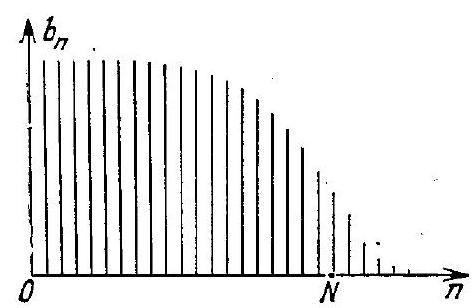
\includegraphics[max width=\textwidth, center]{2024_12_13_2abbd56e24043f80c30dg-5}

Рис. 1.13. Спектр скорости в окрестности сепаратрисы

ранее. Отсюда следует, что спектр нелинейных колебаний маятника имеет вид, приведенный на рис. 1.13 , и число $N$ определяет характерное число гармоник в спектре.

По мере приближения к сепаратрисе $N \rightarrow \infty$, а сам спектр стремится к непрерывному. Как это высказывалось ранее в более общей форме, величина $N$ является параметром характерного обрезания числа гармоник спектра.

Появление расходимости при $\omega \longrightarrow 0$ есть следствие приближения к траектории, проходящей через гиперболическую точку (т. е. к сепаратрисе). Это свойство имеет место не только при $H \rightarrow \omega_{0}^{2}-0$, т. е. снизу, но и при " $H \rightarrow \omega_{0}^{2}+0$, т. е. со стороны пролетных частиц.

Общие свойства периода колебаний. Рассмотрим подробнее, как появляются нулевые или очень малые частоты колебаний, которые, как мы\\
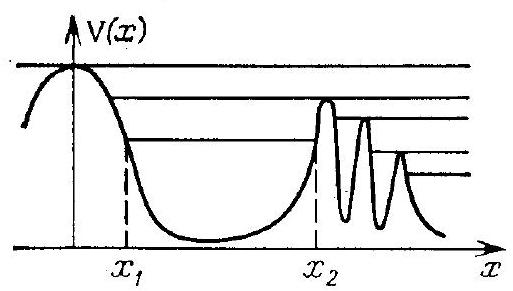
\includegraphics[max width=\textwidth, center]{2024_12_13_2abbd56e24043f80c30dg-5(1)}\\
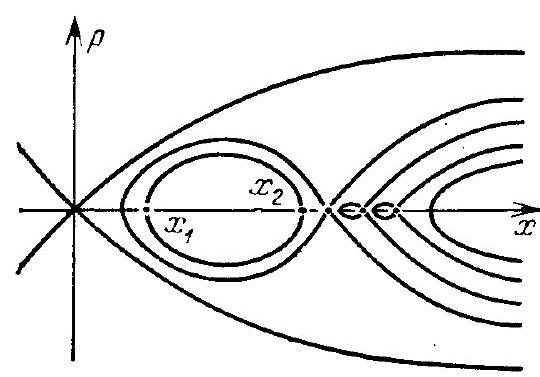
\includegraphics[max width=\textwidth, center]{2024_12_13_2abbd56e24043f80c30dg-5(2)}

Рис. 1.14. Случай нескольких (трех) близких седел

только что видели, радикальнейшим образом изменяют всю картину колебаний по мере удаления от эллиптической точки положения равновесия. Выяснить это важно, так как речь идет о получении более детальной информации о системе при приближении ее траекторий к неустойчивым особым точкам.

Дифференцирование $I$ по $H$ в формуле (2.7) и определение $\omega(1)$ в (2.8) дают период колебаний системы в потенциальной яме:


\begin{equation*}
T=\frac{2 \pi}{\omega}=\oint \frac{d x}{[2(H-V(x))]^{1 / 2}} . \tag{3.22}
\end{equation*}


Исследуем в общей форме это выражение вблизи сепаратрисы. Дл 1 этого обозначим расстояние энергии до сепаратрисы через


\begin{equation*}
\Lambda=\left|H-H_{s}\right| \ll H_{s} . \tag{3.23}
\end{equation*}


Представим знаменатель в (3.22) в виде


\begin{equation*}
[2(H-V(x))]^{1 / 2} \sim\left[\left(x-x_{a}\right)\left(x-x_{b}\right)\left(x-x_{1}\right) \ldots\left(x-x_{n}\right)\right]^{1 / 2} \chi(x) \tag{3.24}
\end{equation*}


где $x_{a}$ и $x_{b}$-точки поворота, между которыми совершается финитное движение; $x_{1}, \ldots, x_{n}$-все другие точки поворэта, кэторы расположәны вблизи, скажем, $x_{b} ; \chi(x)$-функция, не имәющая нулей в комплексной плоскости в окрестности траектории. Для простоты ограничимся случаем, когда все $x_{i}(i=1, \ldots, n)$ - действительные и нули с малой мнимой частью отсутствуют. В примере на рис. $1.14 n=5$.

Основной вклад в выражение для $T$ дают области по $x$ в окрестности полюсов подынтегрального выражения, т. е. нулей импульса (3.24). Близко расположенные нули увеличивают кратность полюса. В окрестности сепаратрисы всегда имеется, по крайней мере, близость к двукратному вырождению: $n \geqslant 1$.

На основании сделанного замечания производим интегрирование в (3.22) только в окрестности полюса. Это дает

\[
T=\frac{2 \pi}{\omega} \sim \frac{2 \pi}{\omega_{0}}\left\{\begin{array}{l}
\ln \left(H_{s} / \Delta\right) \quad(n=1),  \tag{3.25}\\
\left(\Delta / H_{s}\right)^{-(n-1) / 2} \quad(n>1) .
\end{array}\right.
\]

Из формулы (3.25) можно также определить степень нелинейности колебаний:

\[
\frac{d \omega}{d H} \sim \begin{cases}\omega^{2} /\left(\omega_{0} \Delta\right) & (n=1)  \tag{3.26}\\ \omega / \Delta & (n>1)\end{cases}
\]

Удобно выразить последнюю формулу либо только через энергию, либо только через частоту. Имеем


\begin{align*}
& \alpha=\frac{d \omega}{d H} \frac{H_{s}}{\omega_{s}} \sim \frac{H_{s}}{\Delta}\left\{\begin{array}{ll}
1 / \ln \left(H_{s} / \Delta\right) & (n=1) \\
1 & (n>1)
\end{array}\right\}= \\
&= \begin{cases}\left(\omega / \omega_{0}\right) \exp \left(\omega_{0} / \omega\right) & (n=1) \\
\left(\omega_{0} / \omega\right)^{2 /(n-1)} & (n>1)\end{cases} \tag{3.27}
\end{align*}


Наиболее универсальное описание получается в энергетической шкале. Параметр нелинейности стремится к единице по мере роста числа точек поворота $n$, близких к данной точке поворота.
\end{document}